% Due to initial mass requirements of the molecular clouds which collapse to form
% stars, star formation is strongly biased towards lower mass, later spectral
% class stars when compared to higher mass stars. Partly as a result of this
% bias and partly as a result of their extremely long main-sequence lifetimes,
% M-dwarfs make up approximately 70 percent of all stars in the galaxy.
% Moreover, some planet search campaigns have focused on M-dwarfs due to the
% relative ease of detecting small planets in their habitable zones
% \citep[e.g.][]{Nut08}. M-dwarfs then represent both a key component of the
% galactic stellar population as well as the possible set of stars which may host
% habitable exo-planets. Given this key location M-dwarfs occupy in modern
% astronomy it is important to have a thorough understanding of their structure
% and evolution.
%
% \subsubsection{Observations and Instability}
A theoretical explanation for the Jao Gap (Figure \ref{fig:JaoGap}) comes from
\citet{van2012}, who propose that in a star directly above the transition mass,
due to asymmetric production and destruction of He$^{3}$ during the
proton-proton I chain (ppI), periodic luminosity variations can be induced.
This process is known as convective-kissing instability. Such a star will
descend the pre-MS with a radiative core; however, as the star reaches the zero
age main sequence (ZAMS) and as the core temperature exceeds $7\times 10^{6}$
K, enough energy will be produced by the ppI chain that the core becomes
convective. At this point the star exists with both a convective core and
envelope, in addition to a thin, radiative, layer separating the two.
Subsequently, asymmetries in ppI affect the evolution of the star's convective
core.

\begin{figure}
	\centering
	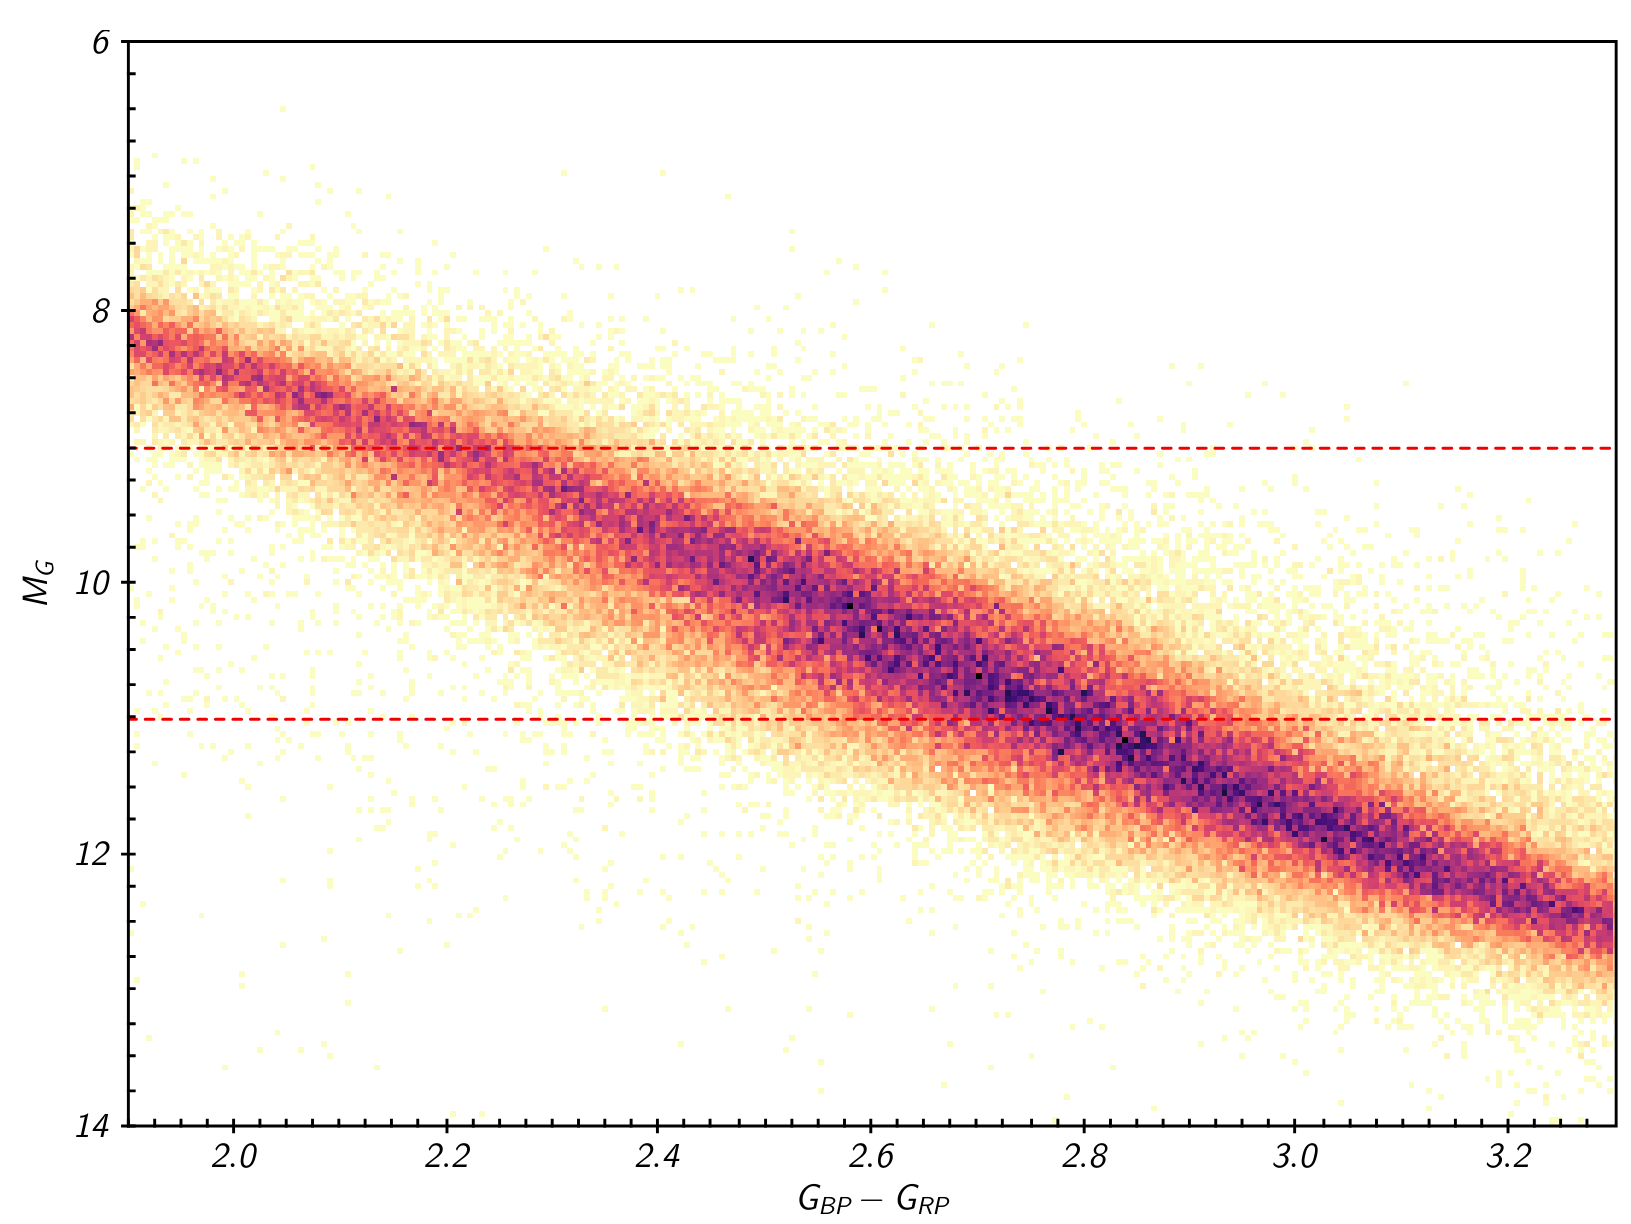
\includegraphics[width=0.75\textwidth]{src/Figures/JaoGap.png}
	\caption{Figure 1 from \citet{Jao2018} showing the so called ``Jao Gap'' at
	$M_{G}\approx$ 10}
	\label{fig:JaoGap}
\end{figure}

The proton-proton I chain constitutes three reactions 
\begin{enumerate} 
	\item $p + p \longrightarrow d + e^{+} + \nu_{e}$
	\item $p + d \longrightarrow \ ^{3}\text{He} + \gamma$
	\item $^{3}\text{He} + ^{3}\text{He} \longrightarrow \ ^{3}\text{He} + 2p$ 
\end{enumerate} 
Because reaction 3 of ppI consumes $^{3}$He at a slower rate than it is
produced by reaction 2, $^{3}$He abundance increases in the core increasing
energy generation. The core convective zone will therefore expand as more of
the star becomes unstable to convection. This expansion will continue until the
core connects with the convective envelope. At this point convective mixing can
transport material throughout the entire radius of the star and the high
concentration of $^{3}$He will rapidly diffuse outward, away from the core,
again decreasing energy generation as reaction 3 slows down. Ultimately, this
leads to the convective region around the core pulling back away from the
convective envelope, leaving in place the radiative transition zone, at which
point $^{3}$He concentrations build up in the core until it once again expands to
meet the envelope.  This process repeats until chemical equilibrium is reached
throughout the star and the core can sustain high enough nuclear reaction rates
to maintain contact with the envelope, resulting in a fully convective star.


\subsubsection{Modeling the Gap}
Since the identification of the Gaia M-dwarf gap, stellar modeling has been
conducted to better constrain its location, effects, and exact cause.
Both \citet{Mansfield2021} and \citet{Feiden2021} identify that the gap's mass
location is correlated with model metallicity --- the mass-luminosity
discontinuity in lower metallicity models being at a commensurately lower mass.
\citet{Feiden2021} suggests this dependence is due to the steep relation of
the radiative temperature gradient, $\nabla_{rad}$, on temperature and in turn,
on stellar mass.

\begin{align}\label{eqn:radGrad}
	\nabla_{rad} \propto \frac{L\kappa}{T^{4}}
\end{align}

As metallicity decreases so does opacity, which, by Equation \ref{eqn:radGrad},
dramatically lowers the temperature where radiation will dominate energy transport
\citep{Chabrier1997}. Since main sequence stars are virialized the core
temperature is proportional to the core density and total mass (Equation
\ref{eqn:TMRelation}). Therefore, if the core temperature where
convective-kissing instability is expected decreases with metallicity, so too
will the mass of stars which experience such instabilities.

\begin{align}\label{eqn:TMRelation}
	T_{c} \propto \rho_{c}M^{2}
\end{align}

This strong opacity dependence presents a slight problem where modeling is 
concerned. With current computational tools it is infeasible to compute opacities on the
fly; rather, Rossland Mean opacity ($\kappa_{R}$) for individual elements must
be pre-tabulated over a wide range of temperatures and densities. These
opacities can then be somewhat arbitrarily mixed together and interpolated to
form opacity lookup-tables. Multiple groups have performed these calculations
and subsequently made tables available to the wider community, these include
the Opacity Project \citep[OP][]{Seaton1994}, Laurence Livermore National Labs
OPAL opacity tables \citep{Iglesias1996}, and Los Alamos National Labs OPLIB
opacity tables \citep{Colgan2016}.

The OPAL opacity tables in particular are very widely used by current
generation stellar evolution programs (in addition to current generation
stellar model and isochrone grids). However, they are no longer the most
up-to-date elemental opacities or numerically precise. Moreover, the generation
mechanism for these tables, a webform, is no longer reliably online.  

Given its strong theoretical opacity dependence, it is reasonable to expect
updated opacity tables to affect, the Jao Gap's mass range. Therefore, as part
of this project we have transitioned DSEP from OPAL high temperature opacities
to opacities based on measurements from Los Alamos national Labs T-1 group
\citep[OPLIB][]{Colgan2016}. This chapter in the thesis will detail the opacity
transition, provide validation of the new opacity tables, and conduct an
in-depth statistical comparison between the locations of Jao Gaps from
populations modeled using both OPAL and OPLIB opacities.

Preliminary work shows populations modeled with OPLIB opacities have Jao Gaps
at consistently lower masses / redder colors than those modeled using OPAL
opacities (Figure \ref{fig:JaoGapOPALOPLIB} and Table \ref{tab:fineMassRange}).
This is in line with expectations based on OPLIB opacities begin uniformly
lower than OPAL opacities for temperature above $10^{6}$ K (Figure
\ref{fig:opacComp}) --- with the lower opacities requiring commensurately lower
core temperatures before radiation dominates energy transport. 

\begin{figure}
	\centering
	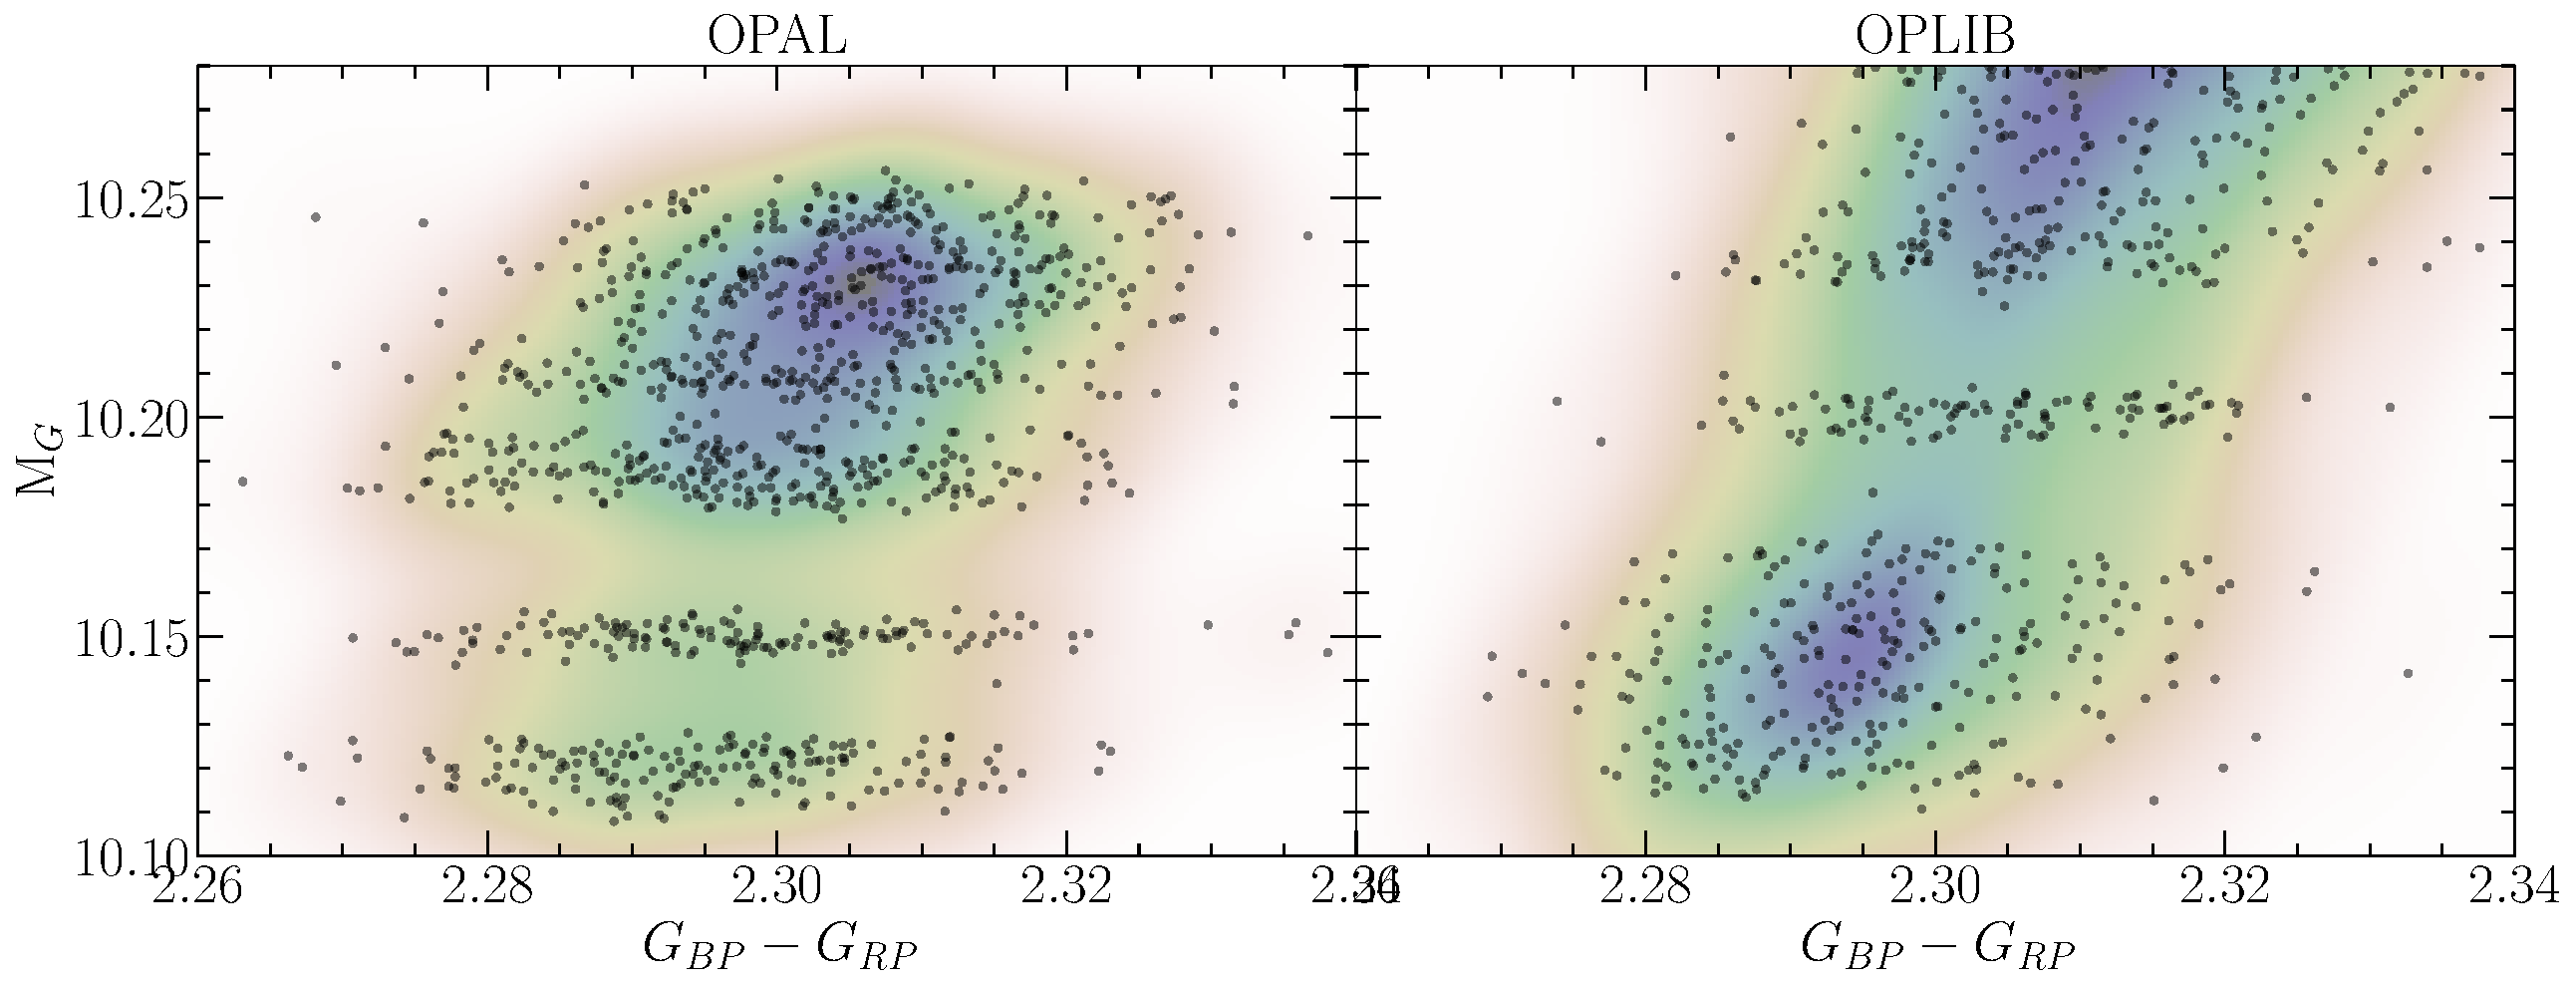
\includegraphics[width=0.85\textwidth]{src/Figures/OPALOPLIB_popsynth_comp.pdf}
	\caption{Synthetic CMDs derived from simple population synthesis code.
	(Left) CMD showing the Jao Gap for a GS98 composition stellar population
	generated from models evolved using OPAL opacity tables. (Right) CMD showing
	the Jao Gap for a GS98 stellar population generated from models evolved
	using the OPLIB opacity tables. Note how the OPLIB derived Jao Gap is
	slightly brighter than the OPAL Jao Gap.}
	\label{fig:JaoGapOPALOPLIB}
\end{figure}

\begin{figure}
	\centering
	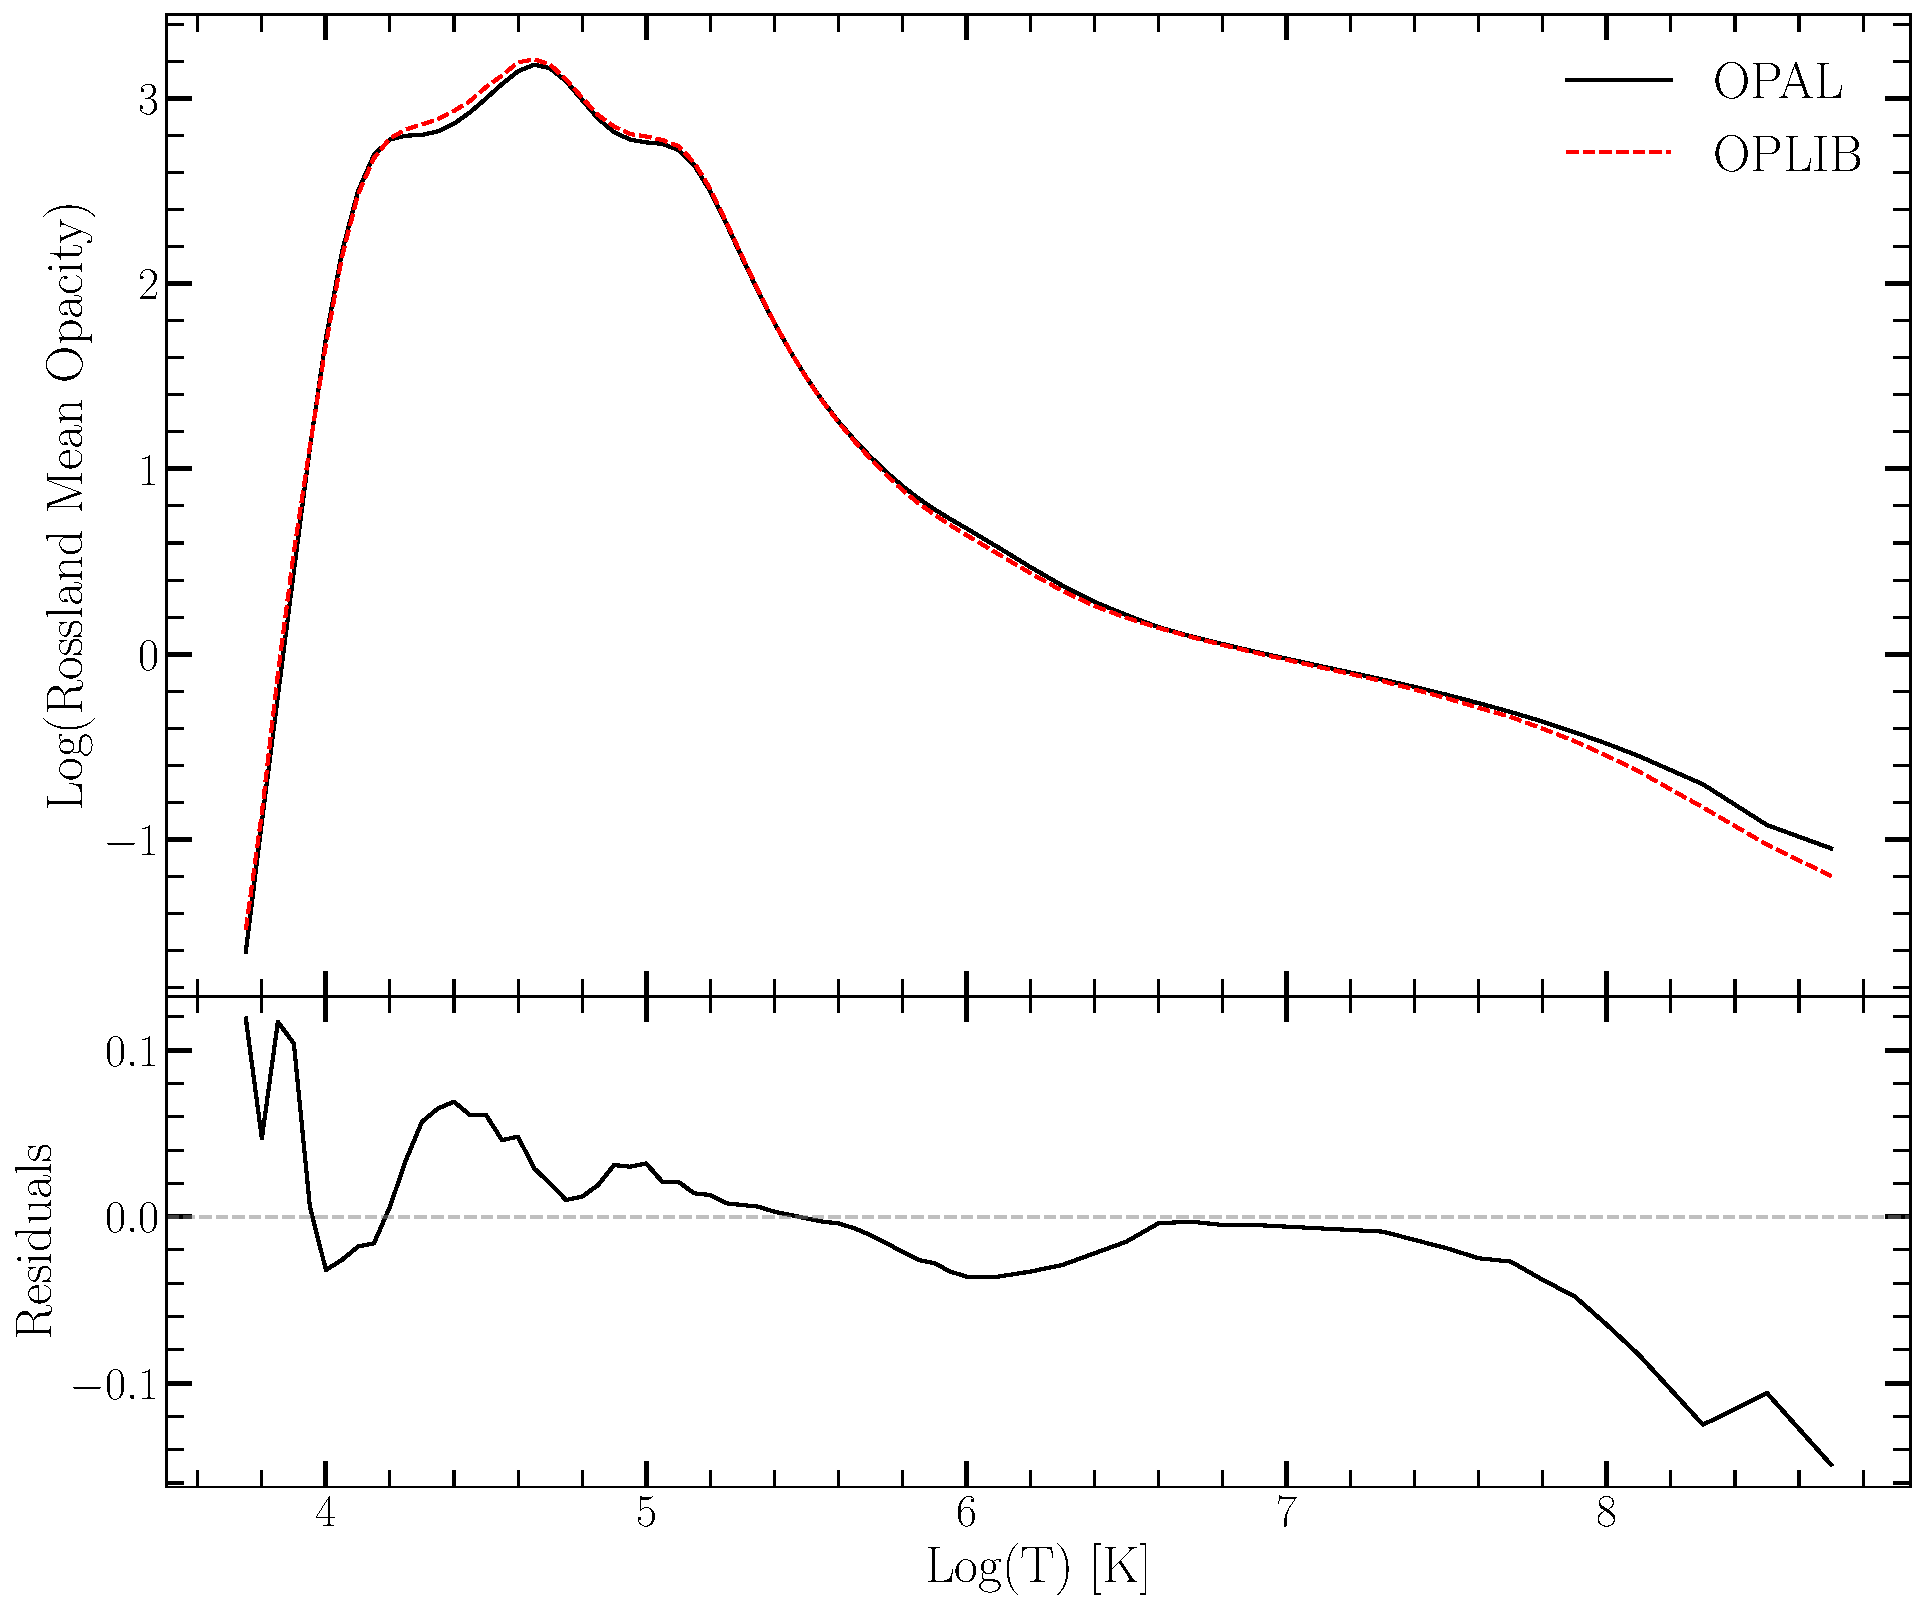
\includegraphics[width=0.75\textwidth]{src/Figures/OpacityComparision.pdf}
	\caption{Rossland Mean Opacity from both OPAL (black solid) and OPLIB (red
	dashed). Note how above 10$^{6}$ K OPLIB opacities are uniformly smaller
	than those from OPAL.}
	\label{fig:opacComp}
\end{figure}

% \subsubsection{OPLIB Opacities}
% In order to address the two main issues with using OPAL opacity tables we use
% our OPLIB opacity table web scraper to generate a set of tables that
% consistently model lower metallicities. Specifically, we generate tables for
% $Z_{\odot}=0.017$, $Z=0.01$, $Z=0.001$, and $Z=0.0001$. Compositions are
% derived from the GS98 solar composition, with the mass fractions between metals
% remaining constant, and only the total metal mass fraction is allowed to vary.
% Moreover, Helium mass fraction is held constant as extra mass from the reduced
% metallicity is put into additional Hydrogen. 
%
% For each metallicity 101, uniformly spaced, models from 0.3 to 0.5 M$_{\odot}$
% (spacing of 0.001 M$_{\odot}$) are evolve with both the GS98 OPAL opacity table
% and OPLIB tables, hereafter these are the ``coarse'' models. For each set of
% coarse models the discontinuity in the mass-luminosity relation is identified
% at an age of 7 Gyr (Figures \ref{fig:coarseMassLum} \& \ref{fig:coarseTeffLum}
% shows a characteristic example).
%
% Immediately, the difference in mass where the discontinuity manifests is clear.
% For each metallicity the discontinuity in the OPLIB models is approximately one
% one-hundredth of a solar mass lower than the discontinuity in the OPAL models. We can
% validate that this discontinuity is indeed correlated with the convective
% transition mass; Figure \ref{fig:convTransition} shows an example of the model
% forming radiative zones at approximately the same masses where the discontinuity
% in the mass-luminosity function exists.
%
% At this resolution only a few models exist within the
% mass range of the discontinuity. In order to better constrain its location we
% run a series of ``fine'' models, with a mass step of 0.0001 M$_{\odot}$ and
% ranging from where the mass derivative first exceeds two sigma away from the
% mean derivative value up to the mass where it last exceeds two sigma away from
% the mean. A characteristic fine mass-luminosity relation is shown in Figure
% \ref{fig:fineMassLum}.


% \begin{figure}
% 	\centering
% 	\vspace{5mm}
% 	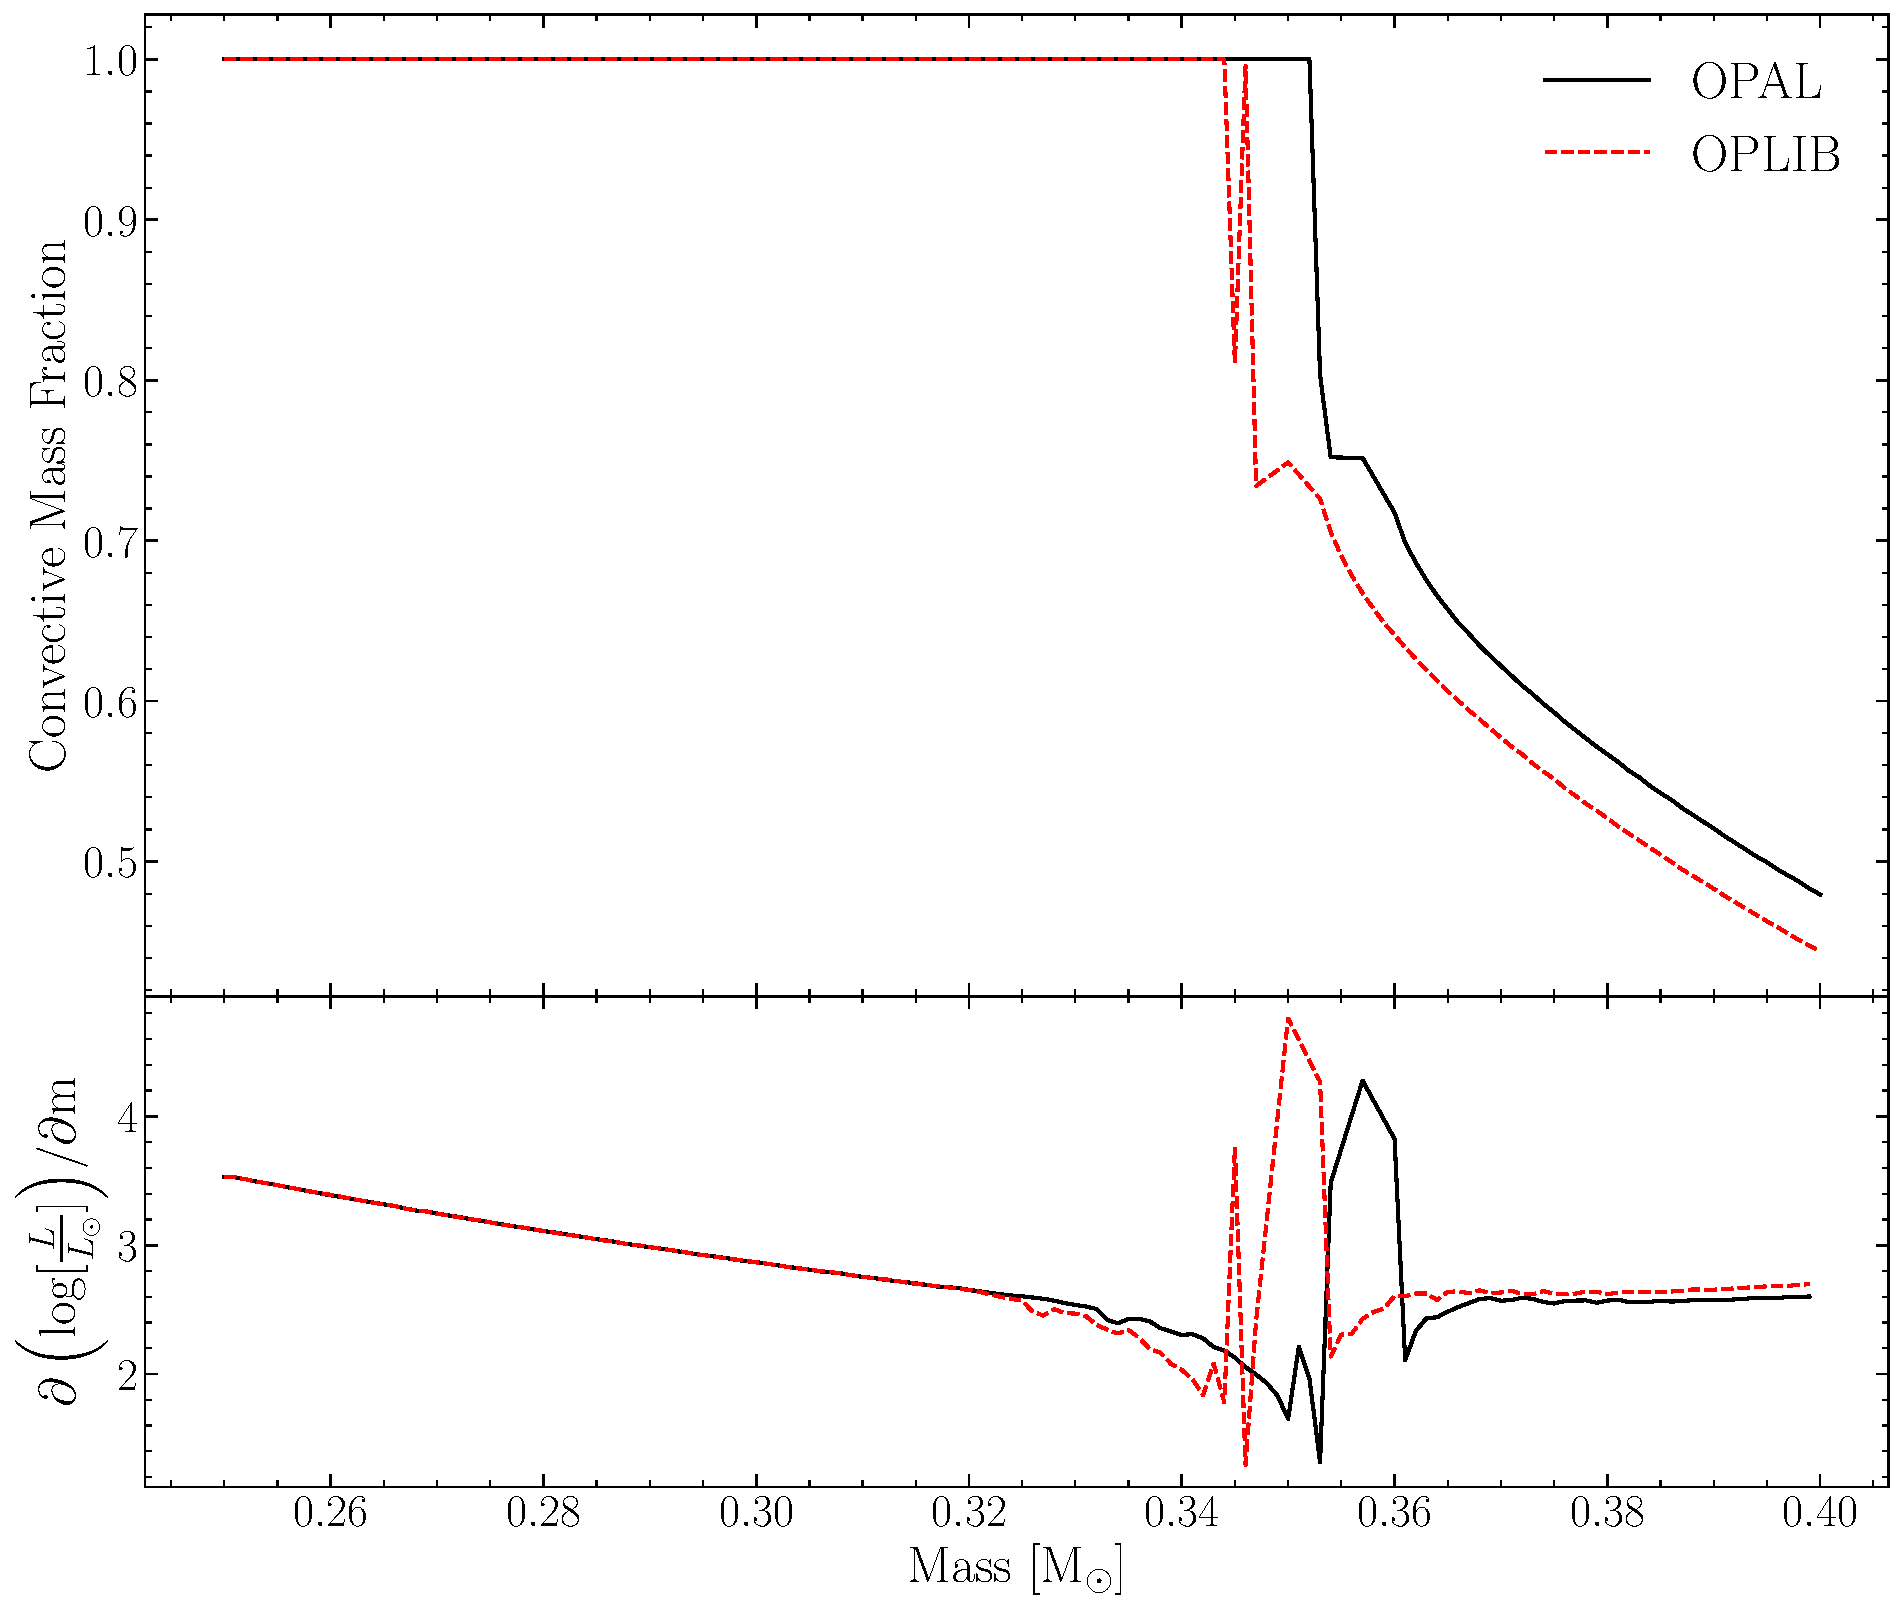
\includegraphics[width=0.45\textwidth]{src/Figures/ConvectiveMassFraction.pdf}
% 	\caption{Convective Mass Fraction vs. initial model mass for Z=0.01 at 7
% 	Gyr (top), Derivative of luminosity with respect to mass for the OPAL and
% 	OPLIB models (bottom).  Note how the model transitions from fully
% 	convective at approximately the same mass where the discontinuity exists.}
% 	\label{fig:convTransition}
% \end{figure}
%
%
% \begin{figure}
% 	\centering
% 	\vspace{5mm}
% 	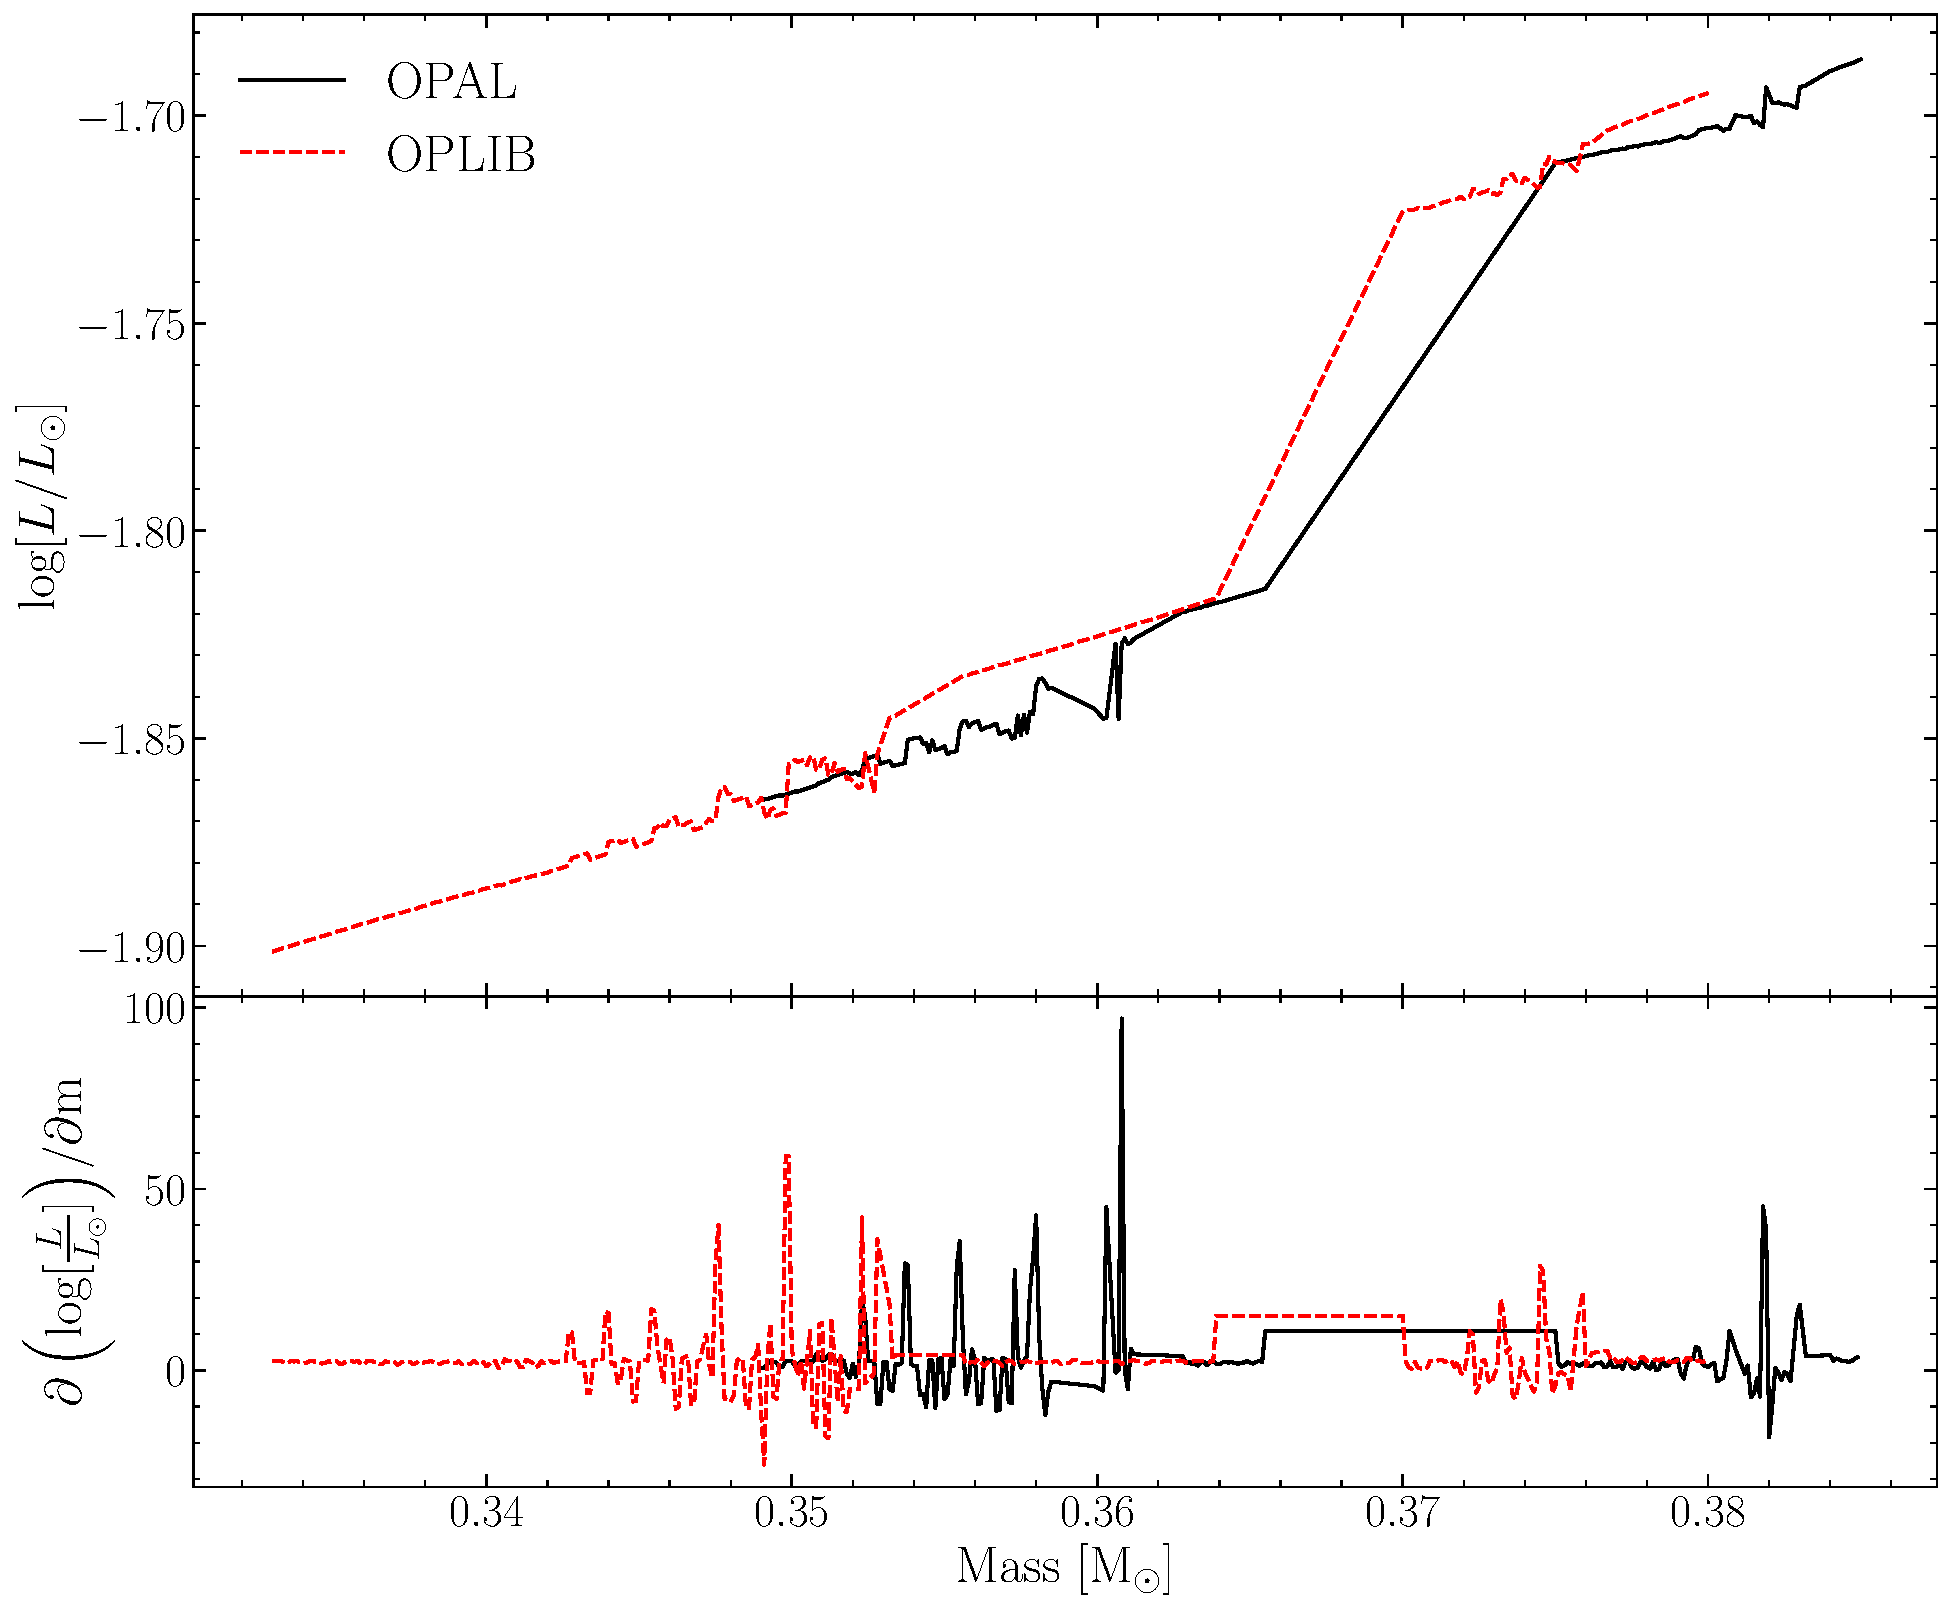
\includegraphics[width=0.45\textwidth]{src/Figures/MassLumDisconZ001Paper-fine.pdf}
% 	\caption{Mass-Luminosity relation for Z=0.01 at 7 Gyr for models run with
% 	both OPAL and OPLIB high-temperature opacity tables and a mass step between
% 	them of 0.0001 M$_{\odot}$ (top). Derivative of luminosity with respect to
% 	mass for the OPAL and OPLIB models (bottom).}
% 	\label{fig:fineMassLum}
% \end{figure}

% Using the fine models we identify the location of the discontinuity in the same
% manner as before, results of this are presented in Table
% \ref{tab:fineMassRange}. Of note with the mass ranges we measure for the
% discontinuity is that are generally not in agreement with those measured in
% \citet{Mansfield2021}. However, the luminosity difference from over the gap
% ($\approx 0.1 mag$) is similar to both the observational difference and that
% reported in \citet{Mansfield2021}. Currently, it is not clear why our mass
% range is not in agreement with the \citet{Mansfield2021} mass range and further
% investigation is therefore needed.

\begin{table*}
	\centering
	\begin{tabular}{r | c c c c}
		\hline
		$Z=$ & Z$_{\odot}$ & 0.01 & 0.001 & 0.0001 \\
		\hline
		\hline
		OPAL & 0.3803 - 0.384 & 0.3583 - 0.3631 & 0.34 - 0.3448 & 0.362 - 0.3663 \\
		OPLIB & 0.374 - 0.3767 & 0.3526 - 0.3567 & 0.3358 - 0.3406 & 0.3577 - 0.3621
	\end{tabular}
	\caption{Mass ranges for the discontinuity in OPAL and OPLIB models. Masses
	are given in solar masses.}
	\label{tab:fineMassRange}
\end{table*}
